			From \eqref{eq:line-rank-2},
the collinearity matrix can be expressed as
 \begin{align}
			    \myvec{-5 & -2
			    \\
			    5 & 2 }  
			    \xleftrightarrow[]{R_2 \leftarrow {R_1 + R_2}}
			    \myvec{	    -5 & -2  
			    \\
			    0 & 0}  
\end{align}
which is a rank 1 matrix. The above process is known as row reduction, where we try to obtain zero rows in the matrix using arithmetic operations.  The number of nonzero rows in the row reduced matrix (also known as {\em echelon form})
is defined as the rank.
		\figref{fig:11/10/2/20}.
	\begin{figure}[H]
		\centering
 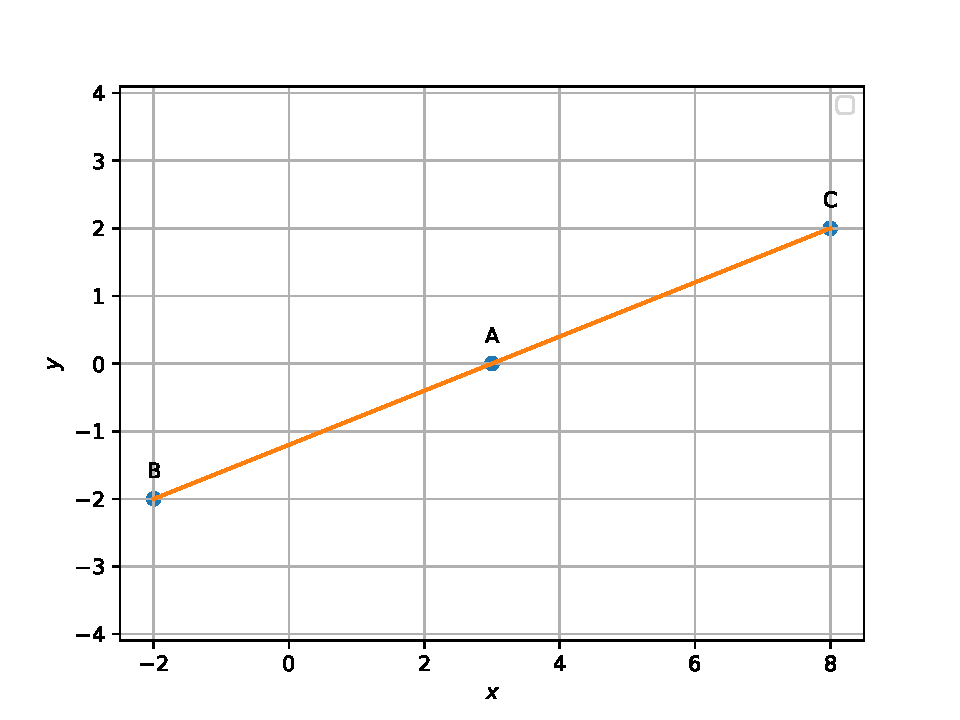
\includegraphics[width=0.75\columnwidth]{chapters/11/10/2/20/figs/figs6.pdf}
		\caption{}
		\label{fig:11/10/2/20}
  	\end{figure}
